\documentclass[12pt,a4paper]{article}
\usepackage[T1]{fontenc}
\usepackage[utf8]{inputenc}
\usepackage{lmodern,amsmath,amssymb,amsthm}
\usepackage[a4paper,margin=25mm]{geometry}
\usepackage{microtype,booktabs,tabularx,array,enumitem,xcolor}
\usepackage{tikz}
\usetikzlibrary{arrows.meta,positioning}
\usepackage[colorlinks=true,linkcolor=blue!45!black,citecolor=blue!45!black,urlcolor=blue!45!black]{hyperref}
\usepackage{listings}
\lstset{basicstyle=\small\ttfamily,columns=fullflexible,keepspaces=true,
breaklines=true,frame=single,rulecolor=\color{black!20},xleftmargin=3pt,xrightmargin=3pt}
\setlength{\emergencystretch}{3em}
\setlength{\parskip}{.25em}
\widowpenalty=10000
\clubpenalty=10000
\setcounter{tocdepth}{1}
\setlist{itemsep=.15em,topsep=.35em}
\newtheorem{theorem}{Theorem}[section]
\newtheorem{lemma}[theorem]{Lemma}
\newtheorem{proposition}[theorem]{Proposition}
\newtheorem{corollary}[theorem]{Corollary}
\theoremstyle{definition}
\newtheorem{definition}[theorem]{Definition}
\newtheorem{example}[theorem]{Example}
\newtheorem{remark}[theorem]{Remark}
\newcommand{\HV}{\operatorname{HV}}
\newcommand{\Mag}{\operatorname{Mag}}
\newcommand{\wtO}{\widetilde O}
\newcommand{\ind}{\mathbf 1}
\newcommand{\R}{\mathbb R}
\newcommand{\N}{\mathbb N}
\newcommand{\Push}{\operatorname{Push}}
\newcommand{\supp}{\operatorname{supp}}
\DeclareMathOperator{\diag}{diag}
\hypersetup{pdftitle={A Numerical Formulation of Chan's Hypervolume Algorithm},
pdfauthor={Michael Emmerich},
pdfsubject={Product measures, exact finite contractions, and preservation of the d/3 exponent}}
\title{A Numerical Formulation of\\Chan's Hypervolume Algorithm}
\author{Michael Emmerich\\[.3em]
\small Technical report accompanying \texttt{FastHVChan}}
\date{5 October 2026\\\small Revised 7 October 2026}
\begin{document}
\maketitle
\begin{abstract}
Hypervolume measures the region dominated by a finite approximation set and
is a central indicator in evolutionary multiobjective optimization. Its
geometric formulation is the union measure of boxes sharing an anchor.
We give a self-contained numerical formulation of Chan's orthant recursion,
written for both optimization and computational geometry readers. The
integrals are evaluated by exact finite cell masses, prefix sums and
monotone integer-cutoff constraints. No quadrature or general symbolic
integration is required. The contribution is an explicit, compilable
numerical implementation of Chan's framework. The simplification is
representational; Chan's own step-function integrals also admit finite
arithmetic evaluation.

The formulation starts directly from ordinary hypervolume under Lebesgue
measure: coordinate weights are interval lengths, while pair constraints
retain geometric dependence. We prove closure under numerical elimination and block-mass
compression, then account for the entire recursive computation. A local
checkpoint policy, optionally skipping compression when the state is
already small, retains Chan's $\wtO_d(n^{d/3})$ arithmetic bound for every
fixed $d\ge4$. Thus the numerical treatment retains the exponent; it does
not improve it. Dimensions two and three use $O(n\log n)$ sweeps.

The accompanying implementation covers dimensions two through ten.
Experiments in 4D--6D use 64--1,024 points, with a 4,096-point 4D stress
test, and compare the proved local policy, an earlier adaptive variant,
and both Python Chan references. Completed timings, partial runs, and
timeouts are kept distinct. Earlier small-input tests remain separate
historical comparisons. The measurements do not establish an asymptotic
exponent or universal practical superiority. An appendix develops the
product-measure extension to dominated-set magnitude and its equivalence
with HV; that extension is not needed by the main algorithm.
\end{abstract}
\vspace{.3em}
\noindent\textbf{Keywords:} hypervolume indicator; Klee's measure problem;
Lebesgue measure; product structure; orthants; numerical elimination;
compression; evolutionary multiobjective optimization.
\newpage
\tableofcontents
\newpage

\section{Purpose, audiences, and the precise claim}
\label{sec:introduction}

In multiobjective optimization, the output of a search is usually a set
of mutually incomparable objective vectors. An indicator assigns a scalar
value to this set, for assessment or for selection during the search.
The hypervolume indicator, introduced by Zitzler and Thiele~\cite{zitzlerthiele1998},
rewards the size of the region dominated by the vectors relative to a
reference point. Repeated indicator evaluations can therefore be a
computational bottleneck. The Wikipedia article~\cite{wikipediahv} gives
an introductory overview; further optimization background is provided
in~\cite{emmerichdeutz2018}.

For computational geometry, the same problem is a restricted union-measure
problem. The boxes share an anchor, equivalently they are orthants clipped
to a bounding box. This restriction is stronger than arbitrary Klee
measure input. Chan's general-box algorithm has an $O(n^{d/2})$ bound,
whereas his orthant framework obtains
$O(n^{d/3}\log^{O_d(1)}n)$ for fixed $d\ge4$~\cite{chan2013}.
The reference implementations in our experiments are named after these
two exponents. A better exponent does not by itself imply a smaller
runtime on a small input.

The objective here is to explain the orthant algorithm using numerical
objects that can be inspected and compiled: ordered coordinate cells,
their masses, monotone cutoff arrays, and signed sums of products.
The presentation preserves the geometric recursion and the compression
that make the bound possible. Simply replacing integrals by sums, or
compiling a slow loop, would not be a sufficient complexity argument.

\paragraph{Attribution and contribution.}
Chan's FOCS paper and its author preprint~\cite{chan2013} provide the
geometric algorithm, the functional framework for its simplification
step, and the $d/3$ exponent. Section~4 of that work describes elimination
through integration and algebraic manipulation of functions. We refer
to this as the symbolic formulation: functions and their integrals are
represented and transformed, rather than only their masses on finite cells.
The FastHVChan implementation project was initiated and developed by
Michael Emmerich. The earlier Python implementation, the numerical
formulation presented here, its software, and the accompanying validation
and benchmarks belong to that implementation project; they are not
software supplied by Chan.

The motivation for this revision was to remove the need to maintain
symbolic functional expressions in an implementation following Chan's
description. The contribution is a compilable numerical implementation,
together with explicit formulas and a proof that its stated compression
policy retains Chan's bound. ``Compilable'' means that the core operations
use numbers and integer-indexed arrays that Numba can translate into
machine code. It does not mean that a symbolic implementation could never
be compiled, nor does it claim a new geometric algorithm or exponent.
The earlier Python reference uses specialized step-function algebra,
not a general-purpose computer algebra package.

\paragraph{For the reader from the Multiobjective Optimization field.}
The main message is that the usual hypervolume indicator can be computed
with interval lengths, prefix sums, and finite array operations, while
retaining Chan's asymptotic bound. The proof explains why the engine
absorbs simple boxes before dividing the remaining instance and why
compression is essential in high dimensions.

\paragraph{For the computational geometry reader.}
The new presentation specializes the functional algebra to a finite
ordered grid of coordinate intervals. Its role is to make the
implementation and its invariants explicit. We provide both a schedule
that charges representation growth and a guarded version of that schedule.
We do not claim a new orthant exponent, a new lower bound, or a new
independent planar factorization.

\paragraph{Origin of the viewpoint.}
The magnitude viewpoint encouraged us to view the problem algebraically;
the earlier \href{https://github.com/emmerichmtm/HV4DMagnitude/blob/main/paper/magnitude_chan_pair_elimination_report.pdf}{report in the HV4DMagnitude repository}
documents that route~\cite{magnitudesoftware}. In the end, the formulation
can be developed directly for the common hypervolume indicator, because
Lebesgue measure itself is a product measure. Magnitude is not required
for the algorithm, its proof, or the measured HV timings.
Appendix~\ref{app:magnitude} contains the metric background, both indicator
transformations, and the additional application of the same engine.

\paragraph{What the complexity statement covers.}
Our main bound applies to the local checkpoint algorithm of
Sections~\ref{sec:geometry}--\ref{sec:complexity}. It includes the fixed
local schedule already used by the standard-library numerical version
and the new compiled local-checkpoint driver. The earlier experimental
compiled driver uses an interval based on the \emph{original} input size.
We do not attach the local-schedule theorem to that different policy.
Section~\ref{sec:software} maps these statements to actual files.

\section{Dominated regions and ordinary hypervolume}
\label{sec:product}

For a finite set $A\subseteq\R_{\ge0}^d$, define
\[
 Q(a)=\prod_{i=1}^d[0,a_i],\qquad
 D(A)=\bigcup_{a\in A}Q(a),\qquad
 \HV_d(A)=\lambda_d(D(A)).
\]
The set $D(A)$ is a down-set in the nonnegative orthant: if $x\in D(A)$
and $0\le y\le x$ coordinatewise, then $y\in D(A)$.
We call $a$ a generator or an upper corner. Repeated or dominated
generators do not change the region. All statements allow tied and zero
coordinates; no general-position hypothesis is needed.

For minimization vectors $p$ and a reference vector $r$ satisfying
$p_i\le r_i$, the conventional region is
$\bigcup_p\prod_i[p_i,r_i]$. The reflection $x\mapsto r-x$ turns it into
$D(\{r-p\})$. This reflection preserves volume, so the upper-corner
convention computes the same hypervolume. The reference point still
determines which region is measured.

For ordinary hypervolume, Lebesgue measure already has product structure:
\[
 \lambda_d=\bigotimes_{i=1}^d\lambda_1,
 \qquad \lambda_d(Q(a))=\prod_i a_i.
\]
This is the algebraic starting point of the algorithm. A union of boxes
need not be a Cartesian product; the geometric constraints must still be
retained. No change of indicator is needed to obtain the product algebra.

\section{Exact discretization and the numerical meaning of an integral}
\label{sec:discrete}

On axis $i$, sort the distinct positive generator coordinates and write
$0=c_{i,0}<c_{i,1}<\cdots<c_{i,m_i}$. Use the cells
\[
 C_{i,0}=\{0\},\qquad C_{i,k}=(c_{i,k-1},c_{i,k}]\quad(k\ge1).
\]
For Lebesgue measure their masses are simply
\[
 w_i(0)=0,\qquad w_i(k)=c_{i,k}-c_{i,k-1}\quad(k\ge1).
\]
The zero cell preserves the rank convention for zero coordinates; it
contributes no ordinary volume. These interval lengths are the only
initial weights required by the HV algorithm.
Every generator becomes a rank vector $r(a)$. Membership in its box is
exactly $k_i\le r_i(a)$ on all axes. Therefore
\begin{equation}
 \HV_d(A)=\sum_{k_1=0}^{m_1}\cdots\sum_{k_d=0}^{m_d}
       \ind[\exists a\in A:\ k\le r(a)]\prod_iw_i(k_i).
 \label{eq:finite-sum}
\end{equation}
This is an exact identity, not a mesh approximation. The algorithm stores
only the separate axis arrays, of total length $O_d(n)$, and structured
constraints. It does not construct the potentially $O(n^d)$ product grid
displayed in the definition of the sum.

Consider a one-dimensional step density $h$ and let $w(k)$ be its
integral over cell $k$. For a union of whole consecutive cells,
\[
          \int_{\bigcup_{k=L}^U C_k}h(x)\,dx
             =\sum_{k=L}^U w(k)=P(U+1)-P(L),
 \qquad P(t)=\sum_{k<t}w(k).
\]
A step-function implementation stores breakpoints, density values, and
an antiderivative represented by cumulative interval contributions.
A cell-mass implementation stores the $w(k)$ and their prefixes directly.
These are two finite arithmetic descriptions of the same operation.

The difference matters in implementation. Integer ranks handle strict
and weak endpoints explicitly, and the bulk operations compile into
loops over typed arrays.
There is no general symbolic-expression manipulation and no quadrature
error. Nevertheless, evaluating a known step-function antiderivative was
already numerical arithmetic in the Python Chan reference. The
simplification is an explicit finite representation, not the elimination
of a computer algebra system that the reference never used.

For a concrete HV example, take $A=\{(2,1),(1,2)\}$.
The axis coordinates are $(0,1,2)$ and the mass arrays are $(0,1,1)$.
The only uncovered positive-area cell within the enclosing square is
$(1,2]\times(1,2]$, indexed by $(2,2)$. Thus the HV is $4-1=3$.
This tiny grid is useful for explanation and testing; the high-dimensional
solver avoids enumerating its analogue.
Appendix~\ref{app:eight} gives a complete eight-point 4D example,
including the actual cuts, a worked numerical leaf, and a separate
illustration of compression.

The finite algebra also accepts supplied masses from another product
measure $\nu=\bigotimes_i\nu_i$: set $w_i(k)=\nu_i(C_{i,k})$ and replace
$\HV_d(A)$ on the left of~\eqref{eq:finite-sum} by $\nu(D(A))$.
The coordinate cells still make each box-membership predicate constant.
This extension changes the initial weights, not the recursive operations.
Its cumulative-coordinate interpretation is given in Appendix~\ref{app:magnitude}.

\section{Why product structure helps, and what remains coupled}
\label{sec:structure}

The product structure of Lebesgue measure lets the initial state be
stored as $d$ unary arrays
instead of a table with one entry per product cell. It also lets us sum
an unconstrained variable by a single scalar factor. Geometry enters
through predicates. After absorbing a two-sided box or eliminating a
variable, the state generally ceases to be one independent product.
It remains a \emph{sum of constrained products}, which is the useful
closure property.

For example, in four dimensions let
\[
 A=\{(2,1,1,1),(1,1,2,1)\}.
\]
Its HV is $3$, but the product of the HVs of the projections on coordinate
pairs $(1,2)$ and $(3,4)$ is $2\cdot2=4$. The projected calculation has
lost the information about which extents occur together in a generator.
Our representation keeps constraints connecting the pairs.

This also explains the scope of a ``$2+2$ split''. In 4D we may eliminate
axes $(1,2)$ and then $(3,4)$. Finite sums justify that grouping without
an independence assumption. The implementation performs the two scalar
eliminations within each pair; it does not provide a separate constant-time
joint planar contraction. For odd $d$, the last coordinate is a singleton.
No dummy dimension is needed.

Another benefit is that compression preserves masses directly. A block
can contain positive-length cells and zero-mass endpoint cells.
Its total mass is a sum. There is no need to divide by a cell's volume or
reconstruct an artificial continuous density. The same finite operations
also work for the supplied product masses described above.

\section{Finite contraction with monotone pair constraints}
\label{sec:contraction}

Let $p$ variables range over finite chains $E_i=\{0,\ldots,s_i-1\}$.
The number $p$ is at most $d$ in a state and at most $2d$ during compression.
A term has the form
\begin{equation}
 T(k)=c\prod_i u_i(k_i)
           \prod_e\ind[k_{j_e}\mathrel{\bowtie_e} f_e(k_{i_e})],
 \qquad i_e<j_e,\quad \bowtie_e\in\{\le,\ge\}.
 \label{eq:term}
\end{equation}
Coefficients and unary arrays may be signed. The integer cutoff arrays
$f_e$ are monotone. For each unordered variable pair we keep four possible
classes: upper or lower inequality, each with a nondecreasing or
nonincreasing cutoff. Same-class upper bounds combine by minimum and
lower bounds by maximum. Cutoffs of opposite monotonicities stay separate.
The sentinels $-1$ and $s_j$ encode impossible upper and lower bounds.

A state $F$ is a sum of $S$ such terms. If $M=\sum_i s_i$, its storage
is $O_p(SM)$; it is not a dense $p$-dimensional array. The signed
representation is an algebraic device. It does not assert that the
underlying initial measure has negative mass.

\subsection{How comparisons stay in this class}
Bounds on a variable are constants or monotone arrays in one other
variable. Consider a comparison $A(k_i)\le B(k_j)$.
If $i=j$, evaluate it entrywise and multiply the resulting Boolean array
into $u_i$. This array need not be monotone. If one side is constant,
the comparison is likewise a unary mask. Otherwise, search the monotone
array associated with the larger-index variable. For a nondecreasing
$B$, for example, $A(k_i)\le B(k_j)$ becomes
\[
 k_j\ge \min\{t:B(t)\ge A(k_i)\},
\]
with an impossible-bound sentinel when the set is empty. Binary searches
handle plateaus and strict inequalities using the appropriate first or
last admissible position. The result is a monotone cutoff array.
Nonincreasing arrays reverse the inequality direction in the same way.
All four classes are needed for closure under these comparisons.

\subsection{First-winner elimination}
To sum out a variable $q$, rewrite each incident predicate as a lower or
upper bound on $q$, inverting its monotone cutoff if needed. Include the
domain endpoints. The feasible interval is
\[
 L(k)=\max_a L_a(k),\qquad U(k)=\min_b U_b(k).
\]
Each candidate depends on at most one surviving variable. Give the
candidates a fixed order. For every pair $(a,b)$, let $G_{ab}$ assert
that $L_a$ is the \emph{first} maximizing lower bound, $U_b$ is the
\emph{first} minimizing upper bound, and $L_a\le U_b$.
For the lower winner, the comparisons with earlier candidates are
strict and those with later candidates weak; the upper winner has the
analogous rule. Thus ties do not create overlaps.

With $P_q(t)=\sum_{r<t}u_q(r)$, the part of the sum on this winner region is
\begin{equation}
 G_{ab}(k)\,[P_q(U_b(k)+1)-P_q(L_a(k))].
 \label{eq:winner}
\end{equation}
All factors in~\eqref{eq:term} that do not involve $q$ remain in place.
Each prefix evaluation in~\eqref{eq:winner} is constant or unary in the
variable supplying its bound. If the two bounds have different source
variables, split the difference into two signed terms; if they have the
same source, one unary difference suffices. In particular, a signed prefix
array is never assumed monotone and is never inverted as a cutoff.

\begin{lemma}[Numerical closure]\label{lem:closure}
Eliminating one of $p$ variables from one term produces at most
\[
                         B_p=2(2p-1)^2
\]
terms of the form~\eqref{eq:term}. For fixed $p$, it costs
$O_p(M\log(M+2))$ arithmetic and comparison operations per incoming term,
apart from optional merging of equal resulting terms.
\end{lemma}
\begin{proof}
Each other variable contributes at most two lower and two upper candidates;
with a domain endpoint there are at most $2p-1$ of each. There are therefore
at most $(2p-1)^2$ winner pairs. Their guards are comparisons of the forms
already described, hence can be represented by unary or pair masks.
The winner regions partition the feasible assignments, and each produces
at most two terms by~\eqref{eq:winner}. A dimension-bounded number of
array scans and binary searches establishes the cost. No new variable
or larger coordinate domain is introduced.
\end{proof}

For a numerical illustration, take $u=(1,2,3,4)$, so
$P=(0,1,3,6,10)$. If the winning bounds are $L=1$ and $U=2$,
the contracted mass is $P(3)-P(1)=6-1=5$. Bounds that depend on other
variables select different entries of this same prefix array.
The winner guards explain how the solver shares that calculation while
retaining the conditions under which those entries apply.

Equal terms may be normalized and merged, and zero terms discarded.
These operations are valuable in practice, but the proof of closure and
the global bound do not assume that cancellation or merging is successful.
This distinction is essential: a small experimental term count cannot
substitute for a worst-case argument.

\section{Compression is a mass-preserving change of index set}
\label{sec:compression}

Suppose $m$ hard boxes remain in a recursive cell. On every axis, put a
block boundary immediately after each hard-box cutoff below the cell's
upper endpoint. The resulting consecutive blocks are
$I_i(t_i)=[\ell_i(t_i),r_i(t_i)]$, with at most $m+1$ blocks per axis.
Define a coarse state by
\begin{equation}
 (\Push F)(t)=\sum_{k_i\in I_i(t_i)\,\forall i}F(k).
 \label{eq:push}
\end{equation}
This is a specification by a finite sum, not an instruction to enumerate
every product of blocks.

For each term, introduce the $d$ new variables $t_i$ with unary weight
one and the comparisons
$\ell_i(t_i)\le k_i\le r_i(t_i)$. There are now $2d$ variables.
Eliminate just the old $k_i$ variables using Lemma~\ref{lem:closure}.
The result is a sum of terms on the block indices. The old variables
can be eliminated in consecutive pairs, with a final singleton for
odd $d$.

\begin{lemma}[Compression and future masks]\label{lem:compression}
If $F$ has $S$ terms and total axis length $M$, the compression emits at
most $C_dS$ terms, where
\[
                       C_d=\prod_{p=d+1}^{2d}B_p.
\]
Its work is $\wtO_d(S(M+m+1))$ before optional merging. The output has
total axis length $O_d(m+1)$ and storage $O_d(C_dS(m+1))$.
For every mask $g$ constant on each product of blocks,
\begin{equation}
             \sum_k F(k)g(k)=\sum_t(\Push F)(t)g(t).
 \label{eq:maskreuse}
\end{equation}
\end{lemma}
\begin{proof}
Apply Lemma~\ref{lem:closure} to the $d$ old variables. The combined
axis length is $M+O_d(m+1)$ and decreases during elimination. Every
surviving unary and cutoff array is indexed by a single coarse axis.
For~\eqref{eq:maskreuse}, partition the sum over the disjoint products
of blocks and move the constant value of $g$ outside each inner sum.
\end{proof}

All surviving hard-box boundaries were used when making the blocks.
Future restrictions and cuts based on these boxes are therefore aligned
with them. Descendants introduce no new original coordinates: clipping
uses current cell boundaries and surviving hard cutoffs. The compression
can consequently be reused throughout the descendant recursion until
another compression is appropriate.

Compression coarsens the coordinate vocabulary. It need not decrease
the number of terms or the total stored entries immediately. The factor
$C_d$ is dimension dependent and can be large. In the actual natural
compression probe, one compression changes one term into 296 terms.
The benefit required by the proof is that the array lengths now depend
on the remaining hard boxes rather than the old coordinate history.
The proof must charge this growth in term count as well as the shorter
arrays.

\section{Geometric recursion and its invariant}
\label{sec:geometry}

At a node, let $\Gamma=\prod_i[l_i,h_i]$ be an inclusive integer-index
cell, $B$ the remaining boxes, and $F$ the numerical state. The quantity
computed is uncovered mass:
\begin{equation}
 U(F,B,\Gamma)=\sum_{k\in\Gamma}F(k)
                          \prod_{b\in B}(1-\ind[k\le b]).
 \label{eq:invariant}
\end{equation}
Initially $F(k)=\prod_iw_i(k_i)$. The final answer is the mass of the
enclosing box minus $U$. After compression, $F$ denotes block masses;
the same invariant still applies.

\subsection{Simplify before cutting}
A box is disjoint if $b_i<l_i$ for some $i$ and can be discarded.
Otherwise, call axis $i$ active if $b_i<h_i$. There are four cases.
\begin{enumerate}
\item With no active axis, the box covers the cell and $U=0$.
\item With one active axis $i$, its covered region is a slab. Its
complement tightens the lower bound to $b_i+1$, or equivalently multiplies
the state by the unary mask $\ind[k_i>b_i]$.
\item For boxes with exactly two active axes $i<j$, combine the group
using a suffix maximum:
\[
 f(k_i)=\max\{b_j:b\text{ in the group},\ b_i\ge k_i\},
 \qquad\max\varnothing=-1.
\]
The group is uncovered precisely when $k_j\ge f(k_i)+1$. This is one
nonincreasing lower cutoff, which can be absorbed into every term.
\item Every remaining hard box has at least three active axes.
\end{enumerate}
Thus simple boxes are replaced by unary or pair constraints. Absorbing
them does not multiply the number of terms. Shared extents produced by
clipping are included automatically; they need not exist in the original
input.

The compiled driver also crops the state to the current cell, removes
constraints that become impossible or tautological on nonzero support,
and merges equal states. These are exact restrictions, not approximations.
All cell endpoints are inclusive. A split after rank $c$ gives
$[l,c]$ and $[c+1,h]$; a slab covering through rank $c$ leaves ranks
starting at $c+1$. Cropping shifts cutoff values by the target-axis
offset. It does not recompute or insert initial cell masses.

\subsection{Why three active axes produce the exponent $d/3$}
Cycle through coordinate axes. At the current axis, let the cyclic
positions of the axes be $0,1,\ldots,d-1$. For each hard box and each
triple $J$ of its active axes, assign weight
\[
                     \omega(J)=2^{\sum_{j\in J}\operatorname{pos}(j)/d}.
\]
Let $\Phi$ be their total weight. For fixed $d$ and nonempty hard input,
$\Phi=\Theta_d(m)$, where $m$ is the number of hard boxes.
Choose a weighted median of the current-axis cutoff coordinates,
using weights of the triples containing that axis, and split after it.
Then advance the cyclic axis. If there are no candidate triples, simply
advance the axis without a cut.

\begin{lemma}[Weighted contraction]\label{lem:potential}
With the exact weights above, each child after a cut and cyclic advance
has potential at most $2^{-3/d}\Phi$. An advance with no candidate has
the same bound and only one child.
\end{lemma}
\begin{proof}
For a triple not using the current axis, the cyclic advance subtracts
three from the sum of its positions, multiplying its weight by
$2^{-3/d}$. A triple using the axis instead increases its position sum
by $d-3$. At most half the current-axis triple weight survives in either
child: in the left child, a cutoff at or beyond the cut becomes inactive;
in the right child, a cutoff at or below the cut is disjoint. Tied cutoffs
at the median therefore cause no ambiguity. The combined factor for these
triples is at most $\tfrac12 2^{(d-3)/d}=2^{-3/d}$.
Restriction and further absorption introduce no new active triples.
When the axis has no candidate, only the first type of triple is present.
\end{proof}

One full round of $d$ advances has at most $2^d$ descendants, each with
potential at most $\Phi/8$. Balancing $2^d$ branches against a size
reduction by $8$ suggests exponent $d/3$. This geometric observation
alone does not bound the work: large numerical histories could still be
carried into all those descendants. Section~\ref{sec:complexity} supplies
the missing accounting.

\subsection{Integer median weights}
Let $n_0$ be the original input size and $A_0=(n_0+2)^2$. Instead of
storing irrational weights, use
\begin{equation}
 W_s=\left\lceil(A_0^d2^s)^{1/d}\right\rceil,
 \qquad 3\le s\le3d-6.
 \label{eq:integerweights}
\end{equation}
Integer power comparisons compute these ceiling roots. They satisfy
\[
 2^{s/d}\le W_s/A_0\le(1+A_0^{-1})2^{s/d}.
\]
Using their weighted median changes the potential contraction by at most
$1+A_0^{-1}$ per advance. Over $O_d(\log(n_0+2))$ advances this has
bounded cumulative effect. For each fixed $d$, sufficiently large $n_0$
ensures $2^{-3/d}(1+A_0^{-1})$ is bounded below one by a
dimension-dependent constant. Smaller inputs lie below a
dimension-dependent constant-size threshold, where the finite grid
gives a bounded number of cuts and axis skips. The integer weights have $O_d(\log(n_0+2))$
bits. Their construction and use add only polylogarithmic work in our
fixed-dimensional arithmetic analysis.

\subsection{Small bases and low dimensions}
If at most a fixed number $b$ of hard boxes remain (the code uses $b=2$),
expand the product in~\eqref{eq:invariant}. Its $2^b$ terms are signed
rectangle sums, each evaluated by numerical elimination. This is
constant-size inclusion--exclusion; it is not an exponential expansion
over all input boxes.

In 2D, a descending first-coordinate sweep needs only the maximum active
second-coordinate prefix mass. In 3D, the same sweep maintains the mass
of a union of anchored rectangles. If $h(y)$ is the active maximum
third-coordinate prefix mass, it is nonincreasing in the second rank.
An inserted rectangle updates a prefix by $h(y)\gets\max(h(y),v)$.
The affected part is one interval: from the first height below $v$ to the
rectangle's last second-coordinate rank. A lazy segment tree locates
that first height and assigns the interval in $O(\log n)$, maintaining
$\sum_y w_2(y)h(y)$. Sorting and all insertions take $O(n\log n)$
and $O(n)$ space. The same argument applies to supplied nonnegative
initial masses.

\section{A local compression policy that retains Chan's bound}
\label{sec:complexity}

\subsection{The checkpoint rule}
A \emph{block} is a consecutive group of geometric advances along a
path. At a block entry, after absorption, let $P$ be the total integer
triple weight from~\eqref{eq:integerweights}, and put
\begin{equation}
 Q=\lceil P/A_0\rceil,\qquad
 L=d\max\left\{1,\left\lfloor\frac{\log_2 Q}{4d}\right\rfloor\right\}.
 \label{eq:localbudget}
\end{equation}
Give the block a budget of $L$ advances. Both cuts and axis skips consume
one advance. At an uncompleted branch where the budget expires, simplify
the node, then either:
\begin{enumerate}
\item compress onto its surviving hard-box blocks; or
\item skip that compression only if the total stored array entries plus
term count are at most $K_d(m+1)$, for a fixed dimension-dependent constant.
\end{enumerate}
In \emph{both} cases compute a fresh budget from the current $Q$.
The implementation uses the equivalent threshold
$\texttt{compress\_factor}\,d^2(m+2)$ with a fixed finite nonnegative
factor (default eight). Taking factor zero forces compression at each
checkpoint; it does not change the local checkpoint positions.

The skip is justified by a certificate about current storage. It is not
an arbitrary postponement. Resetting the budget even after a skip is
what keeps the next checkpoint local to the smaller subproblem.

\begin{center}
\begin{minipage}{.97\linewidth}
\begin{lstlisting}[caption={Local-checkpoint recursion; all cell bounds are inclusive.},label={alg:local}]
Solve(B, F, cell, axis, remaining):
    discard disjoint boxes; tighten slabs; crop F
    absorb two-sided groups as monotone pair masks
    if a box covers the cell or F is zero: return 0
    if at most b hard boxes remain: return Base(B, F, cell)

    if remaining == 0:
        if stored_size(F) > fixed_factor*d*d*(len(B)+2):
            F = Push(F, blocks at hard-box cutoffs)
            reindex B and cell onto the block axes
        remaining = unset    # reset even after a skip
    if remaining is unset:
        remaining = local_budget(current weighted potential)

    if the current axis has no eligible hard cutoff:
        return Solve(B, F, cell, next_axis, remaining-1)
    c = weighted_median(current-axis hard cutoffs)
    return Solve(left of c,  next_axis, remaining-1)
         + Solve(right of c, next_axis, remaining-1)
\end{lstlisting}
\end{minipage}
\end{center}

\begin{theorem}[Numerical Chan bound with guarded compression]
\label{thm:main}
For fixed $d\ge4$ and fixed base size, the local-checkpoint algorithm
computes the ordinary hypervolume of a union of $n$ anchored boxes in
\begin{equation}
                   O_d(n^{d/3}\log^{c_d}(n+2))
                       =\wtO_d(n^{d/3})
 \label{eq:mainbound}
\end{equation}
arithmetic and comparison operations, for a constant $c_d$ depending
only on $d$. This holds with compression at every checkpoint, or with
the certified skip rule above. Initial coordinate sorting and interval
length construction are included. The same bound applies to a supplied
product measure whose cell masses take $O_d(n\log n)$ work to obtain.
For $d=2,3$, the sweeps give $O(n\log n)$.
\end{theorem}

\begin{proof}
\emph{Correctness.} Discretization is exact by~\eqref{eq:finite-sum}.
Absorption preserves~\eqref{eq:invariant}; inclusive splitting partitions
the cell disjointly. The base case is finite inclusion--exclusion followed
by exact contractions. Lemma~\ref{lem:compression} preserves all later
block-aligned restrictions. Skipping a compression leaves the state
unchanged. Induction on the recursion proves the returned mass is correct.

\emph{Representation at a block entry.} Let $N=\Phi$ after absorption,
$m$ be the hard-box count, $S$ the term count, and $M$ the total length of
the common axis domains. At every nonroot block entry,
\[
                       m=\Theta_d(N),\qquad M=O_d(N+1).
\]
After compression the second relation follows from the $m+1$ blocks per
axis. After a skip it follows from the storage certificate: a nonempty
term contains a unary array for every live axis, so $M$ is no greater
than the certified total storage. Within a block, clipping and absorption
do not lengthen domains or increase $S$. Compression multiplies the term
count by at most $C_d$ from Lemma~\ref{lem:compression}.

\emph{One block.} Since $Q=\Theta_d(N)$, for sufficiently large $N$ the
budget is $L=\tfrac14\log_2N+O_d(1)$. The block contains
$O_d(N^{1/4})$ nodes and leaves. At a surviving child checkpoint,
Lemma~\ref{lem:potential} and the bounded integer-weight perturbation give
\[
                 N'\le c_dN^{\beta},\qquad
                 \beta=1-\frac{3}{4d}<1.
\]
Each node can be charged $\wtO_d(S^2N)$, including coordinate scans,
cut selection, contraction at an early base, or compression at a leaf.
The square is a conservative deterministic allowance for comparing and
merging terms; omitting merging gives a linear dependence on $S$.
Thus the whole block costs $\wtO_d(S^2N^{5/4})$. In particular, no claim
about beneficial cancellation is used.

\emph{Number of blocks and term growth.} Above a sufficiently large
fixed threshold, the recurrence $N'\le c_dN^\beta$ gives
$G=O_d(\log\log(n+2))$ block generations on a path. Below that threshold,
only a constant number of geometric advances remains: the potential
contracts by a fixed factor, and a hard box has a fixed positive minimum
triple weight. Consequently,
\[
                S\le C_d^G=\log^{O_d(1)}(n+2)
\]
along every path from the one-term initial state. Skipped checkpoints do
not increase $S$ and do not invalidate the bound on generations, because
they too restart the local budget.

\emph{Summing the work.} Up to factors depending only on $d$, at
macro-depth $g$ a subproblem size is bounded by $cN_0^{\beta^g}$, and
the number of block entries is at most
\[
 a_d^g N_0^{\frac14\sum_{j<g}\beta^j}
       =a_d^g N_0^{\frac d3(1-\beta^g)}.
\]
Constants raised to $g$, as well as $S^2$, are polylogarithmic in $n$.
The sum of block costs at that depth is therefore bounded, up to such
factors, by
\[
 N_0^{\frac d3(1-\beta^g)+\frac54\beta^g}
  =N_0^{\frac d3-(\frac d3-\frac54)\beta^g}
  \le N_0^{d/3},
\]
since $5/4<d/3$ for every $d\ge4$. Summing over all macro-depths adds
only a polylogarithmic factor.

\emph{The root and low dimensions.} Many boxes can be absorbed at the
root while its arrays still have length $O_d(n)$. Its first block costs
at most $\wtO_d(nN_0^{1/4})\le\wtO_d(n^{5/4})$, with $S=1$, or
$\wtO_d(n)$ if it ends immediately. Both fit~\eqref{eq:mainbound}.
Subsequent block entries obey the invariant already proved. The 2D and
3D sweep analysis supplies their separate bounds; substituting $d=3$
into this block-work calculation would not be justified.
\end{proof}

\subsection{Meaning of the retained exponent}
The proof is a numerical realization of Chan's simplification,
elimination, and compression framework~\cite{chan2013}. His functional
closure and grid-preserving simplification appear in Lemmas 4.4 and 4.5;
the orthant bound is in Section 4.2. Our local schedule makes the
representation-growth charge explicit and permits the storage-certified
skip. The finite prefix operations cause no extra polynomial factor in
$n$. In particular, 4D remains $\wtO(n^{4/3})$.

\begin{center}
\begin{tabular}{@{}clcc@{}}
\toprule
$d$ & Elimination grouping & Arithmetic bound & Lift variables\\\midrule
2 & numerical sweep & $O(n\log n)$ & ---\\
3 & sweep and skyline tree & $O(n\log n)$ & ---\\
4 & $2+2$ & $\wtO(n^{4/3})$ & 8\\
5 & $2+2+1$ & $\wtO(n^{5/3})$ & 10\\
6 & $2+2+2$ & $\wtO(n^2)$ & 12\\
7 & $2+2+2+1$ & $\wtO(n^{7/3})$ & 14\\
8 & $2+2+2+2$ & $\wtO(n^{8/3})$ & 16\\
9 & $2+2+2+2+1$ & $\wtO(n^3)$ & 18\\
10 & $2+2+2+2+2$ & $\wtO(n^{10/3})$ & 20\\
\bottomrule
\end{tabular}
\end{center}
The theorem is fixed-dimensional: its hidden constants and logarithmic
exponents may depend substantially on $d$. It is an arithmetic-operation
bound, not a rational bit-complexity result or a floating-point stability
theorem. It concerns total indicator evaluation, not all exclusive
contributions, gradient evaluation, or online update sequences.

\subsection{Why the older adaptive timings do not prove this theorem}
The earlier compiled adaptive driver uses a level interval of roughly
$0.1d\log_2n_0$, based on the original input size, combined with a size
threshold. This does not restart local blocks at every smaller subproblem
or skipped checkpoint. Moreover, even a locally chosen
$0.1d\log_2N$ interval would give the crude block-work exponent $1+0.1d$,
which is $1.4>4/3$ in 4D. The constant in~\eqref{eq:localbudget} is
deliberate: block work grows like $N^{5/4}$, strictly below the target
exponent in all dimensions under discussion.

Accordingly, the statement ``the numerical treatment retains Chan's
complexity'' is proved here for an explicit numerical algorithm and its
local policy. It is not inferred from a familiar algorithm name, a
compilation setting, or timing plots for a different policy.

\section{Software realization and validation of the local policy}
\label{sec:software}

The repository~\cite{software} provides three relevant variants in
\texttt{NumericalChanHVND}. They share the finite-mass problem formulation
but should not be conflated.
\begin{enumerate}
\item \texttt{numerical\_chan.py} is the standard-library numerical
implementation with locally chosen blocks and compression at each
checkpoint. Integer and \texttt{Fraction} inputs can be evaluated with
exact arithmetic. It is covered by the fixed-local-policy case of
Theorem~\ref{thm:main}.
\item \texttt{numerical\_chan\_compiled.py} is the previously published
compiled adaptive driver. It adds cell pruning and native contractions,
with the global-interval policy discussed above. The archived performance
comparisons measure this variant.
\item \texttt{numerical\_chan\_local\_compiled.py} is the local-checkpoint
compiled driver accompanying this report. It reuses the same native
kernel, cell restriction and base routines, and changes the scheduling
to Listing~\ref{alg:local}. Theorem~\ref{thm:main} covers its algorithmic
policy, with fixed base size and compression factor, under the stated
arithmetic-operation model.
\end{enumerate}
All three support every integer dimension from two through ten. The
theory is for any fixed dimension; ten is an implementation and testing
range, not a mathematical barrier.

\subsection{What is compiled}
The file \texttt{compiled\_terms.py} stores coefficients, unary arrays,
and pair constraints in typed native states. Numba compiles complete
restriction, masking, variable elimination, state merging, base sums,
and block compression. The geometric recursion remains readable Python.
In 2D and 3D the numerical sweeps are compiled instead. The earlier hybrid
Numba version compiled only smaller array helpers while Python retained
much of the term construction and dispatch overhead.

The kernel does not enable fast-math or parallel execution. Coefficients
and unary masses are binary64 values, cutoff indices are integers, and
median weights are the separately constructed Python integers. Dictionary
copies share arrays only while those arrays are immutable; modifications
allocate replacement arrays. State hashes are checked against full
contents before equal terms are merged. Hash collisions cannot justify
an algebraic equality. A limit on collision-chain comparisons may leave
equivalent terms unmerged, which preserves their sum and does not affect
the raw-emission proof.

Compilation changes the cost of an operation, not the identity it
evaluates. Reusing the native kernels under the local policy does not
require a new elimination rule. Conversely, enabling Numba does not
establish either exact real arithmetic or numerical stability. Signed
cancellation can magnify floating-point errors even when the final
indicator is positive.

\subsection{Minimal use}
From the repository root, in an environment with NumPy and Numba:
\begin{lstlisting}[language=Python]
from NumericalChanHVND.numerical_chan_local_compiled import (
    hypervolume, NumericalChanLocalCompiled)

points = [(2, 1, 1, 1), (1, 2, 1, 1)]
assert abs(hypervolume(points) - 3.0) < 1e-10

solver = NumericalChanLocalCompiled(dimension=4)
value = solver.compute(points)
print(solver.stats)
\end{lstlisting}
For minimization data, replace each point by its nonnegative extent
vector $r-p$ before calling the solver. The public validation rejects
negative or nonfinite extents. An empty input and a single all-zero
generator both have HV zero. No dominance filter is required for correctness.

The local driver intentionally exposes no global interval or
compression-disable option. Its compression factor is a fixed constant
in the theorem; factor zero means compression at every scheduled
checkpoint. Arbitrarily changing the block budget or making policy
parameters depend on input size is outside the stated theorem.

\subsection{Validation of the newly proved policy}
The script \texttt{verify\_local\_compiled.py} and its saved JSON record
check the new driver independently of the old timing experiment. They
include 232 exact small-instance checks across dimensions 2--10, 24
additional exact checkpoint-recursion instances, and 3,538 observed
cyclic-advance and budget invariants. Additional product-measure checks
are described in Appendix~\ref{app:magnitude-software}. The trace checks that a skipped axis consumes a step and that
a checkpoint resets its budget after either decision.

A 64-point four-dimensional permuted antichain reaches two successive
checkpoint generations. With factor zero it executes 63 compressions;
with a sufficiently large fixed factor it executes 63 certified skips.
Both settings agree with the independent Chan $d/2$ reference for HV. These deliberately chosen settings validate both branches of
the policy; they are not performance recommendations.

The common-extent 1,552-box family described in
Section~\ref{sec:archived} also executes six \emph{default local-policy}
compressions. Its HV is $6\,372\,330\,876$, agreeing with the independent
Chan $d/2$ computation. These six events occur on different branches; this
case alone does not demonstrate repeated compression on one path.

All checks pass with maximum scaled discrepancy
$5.6844\times10^{-13}$, using relative tolerance $2\times10^{-9}$ and
absolute tolerance $2\times10^{-10}$. Cached import in a fresh process
is also checked. The shared kernel's separate suite tests signed states,
all cutoff orientations, inclusive crops, repeated
compression, and parent-state immutability. These tests corroborate the
implementation; the complexity conclusion rests on
Theorem~\ref{thm:main}, not on a finite test set.

\section{Benchmarks: numerical Chan and two references}
\label{sec:experiments}

The comparison uses three implementations throughout:
\begin{itemize}
\item \textbf{Numerical Chan (Numba):} the implementation described in this
report, with the local compression policy covered by Theorem~\ref{thm:main}.
\item \textbf{Chan $d/3$ (Python):} the repository's implementation following
Chan's functional formulation, with the same theoretical exponent.
\item \textbf{Chan $d/2$ (Python):} the simpler geometric algorithm, included
as a practical baseline despite its larger exponent.
\end{itemize}
These are comparisons of complete implementations. The numerical kernels
are compiled, while the two references run in Python; a timing advantage
therefore does not establish a better asymptotic algorithm.
Older implementation variants are documented in the repository archive
linked in Appendix~\ref{sec:archived}.

\subsection{Inputs and timing protocol}
Here $n$ is the number of input points, each defining one anchored box.
We use two families of positive, mutually nondominated points. Sphere
coordinates are absolute Gaussian samples plus $0.01$, normalized to
Euclidean length one. Simplex coordinates are exponential samples plus
$0.01$, normalized to sum to one. There is one seeded sample per family
and dimension; smaller inputs are prefixes of the largest sample.
The sphere family uses $n=64,128,256,512,1024$ in 4D--6D, plus $4096$ in
4D. The simplex family uses $n=64,256,1024$ in each dimension.

Each fresh worker runs one first call followed by three timed calls,
with a new solver on each call. The tables report the median of the
three timed calls in \emph{seconds}. Input conversion and preprocessing
are included; imports and the first call are excluded. Existing
compilation caches are retained. Compression uses the default settings;
there is no dominance prefilter, fast-math, or concurrent numerical worker.

The 45-second limit applies to the whole worker, including imports and
all four calls. Thus TO means the worker exceeded that budget before completing all
three timed calls; it is not a 45-second lower bound on one call. NR means not run after two smaller-size timeouts in the same
solver/family/dimension series. Partial samples remain available in the
raw data but are not presented as complete medians.

The environment is Windows 11 on an AMD Ryzen 7 5800H with 16 logical
CPUs, Python 3.12.14, NumPy 2.5.3 and Numba 0.68.0. CPU affinity was not
fixed and ordinary system load was uncontrolled. The measured solver
sources are unchanged from revision \texttt{095fa73}; the archived hashes
identify the exact files and inputs.

\subsection{Results and their scope}
Tables~\ref{tab:larger-sphere} and~\ref{tab:larger-simplex} retain every
planned input size. Across the three displayed methods there are 75
algorithm/input rows: 56 complete workers, 18 timeouts, and one not run.
Numerical Chan completes 18 of its 25 rows.

\begin{table}[p]
\centering\small
\setlength{\tabcolsep}{5pt}
\begin{tabular}{rrrrr}
\toprule
$d$ & $n$ & \shortstack{Numerical Chan\\Numba} & \shortstack{Chan $d/3$\\Python} & \shortstack{Chan $d/2$\\Python} \\
\midrule
4 & 64 & 0.0518 & 0.1243 & 0.0245 \\
4 & 128 & 0.1431 & 0.3472 & 0.0684 \\
4 & 256 & 0.3427 & 0.8913 & 0.1622 \\
4 & 512 & 0.8485 & 2.1206 & 0.3859 \\
4 & 1024 & 3.4890 & 4.7949 & 0.8810 \\
4 & 4096 & TO & TO & 4.5595 \\
5 & 64 & 0.2208 & 0.6844 & 0.0878 \\
5 & 128 & 0.6220 & 1.9354 & 0.2568 \\
5 & 256 & 1.9115 & 6.0686 & 0.8202 \\
5 & 512 & 5.2159 & TO & 2.0171 \\
5 & 1024 & TO & TO & 5.0315 \\
6 & 64 & 0.7754 & 3.0187 & 0.2772 \\
6 & 128 & 3.0644 & 10.9978 & 1.2158 \\
6 & 256 & 10.3680 & TO & 3.9232 \\
6 & 512 & TO & TO & TO \\
6 & 1024 & TO & NR & TO \\
\bottomrule
\end{tabular}
\caption{Sphere fronts at larger input sizes: warm median \emph{seconds}. All three methods use the same inputs. TO and NR are defined in the text.}
\label{tab:larger-sphere}
\end{table}

\begin{table}[p]
\centering\small
\setlength{\tabcolsep}{5pt}
\begin{tabular}{rrrrr}
\toprule
$d$ & $n$ & \shortstack{Numerical Chan\\Numba} & \shortstack{Chan $d/3$\\Python} & \shortstack{Chan $d/2$\\Python} \\
\midrule
4 & 64 & 0.0589 & 0.1566 & 0.0262 \\
4 & 256 & 0.3693 & 0.9423 & 0.1621 \\
4 & 1024 & 4.0905 & 5.4955 & 0.9622 \\
5 & 64 & 0.2168 & 0.7958 & 0.1137 \\
5 & 256 & 2.1954 & 7.7507 & 0.9182 \\
5 & 1024 & TO & TO & 6.1703 \\
6 & 64 & 0.8562 & 3.2904 & 0.3552 \\
6 & 256 & TO & TO & 5.2442 \\
6 & 1024 & TO & TO & TO \\
\bottomrule
\end{tabular}
\caption{Simplex fronts at larger input sizes: warm median \emph{seconds}. All three methods use the same inputs. TO and NR are defined in the text.}
\label{tab:larger-simplex}
\end{table}

On the 16 pairs with complete medians for both Numerical Chan and Chan
$d/3$, Numerical Chan is faster in all 16; the median ratio of reference
time to numerical time is $2.88$. Chan $d/2$ is faster on all 18 complete
pairs with Numerical Chan. These summaries omit incomplete runs and
must not be extrapolated to larger inputs.

The 4D sphere with $n=4096$ illustrates this limitation: Numerical Chan
returns its first value in $42.565$ seconds, compared with $23.367$
seconds for Chan $d/3$. Neither completes the three timed repetitions.
These are first-call observations, possibly including native-kernel
initialization and cache loading, not warm medians or empty-cache
compilation measurements.

The displayed methods return 242 first-call and subsequent values.
All agree with an available Chan $d/2$ value within the comparison
tolerance; the maximum scaled error is $3.3307\times10^{-16}$, using
$|v-v_{\mathrm{ref}}|/\max(1,|v_{\mathrm{ref}}|)$. No returned value is
unverified. These larger cases use cross-implementation checks, not
an exponential exact oracle. The separate small-instance checks are
described in Section~\ref{sec:software}.

Four completed Numerical Chan inputs execute compression. Among its
complete workers, the slowest/fastest warm-call ratio has median $1.05$
and maximum $1.26$. With only three repetitions and one sample per
family/dimension, the experiment does not establish an asymptotic
exponent or universal practical superiority. The complexity statement
rests on Theorem~\ref{thm:main}.

Full coordinates, individual timings, partial calls, compression counters,
and source hashes remain in \texttt{benchmarks/larger\_4d\_6d/results}.
The \href{https://github.com/emmerichmtm/FastHVChan/blob/main/NumericalChanHVND/benchmarks/larger_4d_6d/RESULTS.md}{benchmark summary}
uses the same three-method comparison as this report.
\clearpage

\section{Structural validation and archived measurements}
\label{sec:archived}

\paragraph{A structural input for compression.}
The 1,552-box family used in the validation has the following explicit
construction. For each of the six coordinate pairs in 4D, take 256
corners with pair extents $(t,257-t)$, $1\le t\le256$, and extent 300
in the other coordinates. Add 16 corners
$(161+i,176-i,161+j,176-j)$, where $0\le i<16$ and $j=3i\bmod16$.
The first 1,536 corners become pair constraints, leaving long arrays
with relatively few hard boxes. Shared extents are deliberate.

The current Numerical Chan driver executes six default-policy compressions
on this family and returns $6\,372\,330\,876$, agreeing with Chan $d/2$.
These events occur on different branches; they do not by themselves
test repeated compression along one path. The separate checkpoint
tests in Section~\ref{sec:software} cover that case.

An earlier recorded run on this same family illustrates the storage
effect mentioned in Section~\ref{sec:compression}: its first compression
changes one term into 296 terms and increases the stored-entry count
from 1,710 to 6,936. Compression shortens the coordinate histories but
need not immediately shrink the whole representation. These historical
event counts are not runtime measurements of the current driver.

\paragraph{Where to find the earlier experiments.}
The repository preserves the
\href{https://github.com/emmerichmtm/FastHVChan/blob/main/NumericalChanHVND/benchmarks/compiled_2d_10d/RESULTS.md}{earlier 2D--10D comparison}
at solver revision \texttt{38587e7}, including its small inputs, exact
oracle checks and compression probes. The larger experiment also retains
an \href{https://github.com/emmerichmtm/FastHVChan/blob/main/NumericalChanHVND/benchmarks/larger_4d_6d/RESULTS_ALL_VARIANTS.md}{all-variant detail report}.
Its extra implementation is an earlier compiled driver with a different
compression schedule. Those measurements remain available for
reproducibility; they are not included in this paper's main timing tables.

Raw inputs and results have not been changed or recomputed. The totals
in Section~\ref{sec:experiments} count only its three displayed methods;
the full archived experiment has additional rows and therefore different
aggregate counts. The current numerical method's complexity is justified
by the local policy and proof in Section~\ref{sec:complexity}, rather
than by historical timings or compilation alone.


\section{Structural simplifications and limits}
\label{sec:discussion}

The structural simplification can be stated precisely. Initially a
product measure is stored as one unary factor per axis. Local geometric
simplification replaces one- and two-sided boxes by unary and monotone
pair predicates. Summing one variable introduces only a fixed-dimensional
number of terms of the same form. Compression replaces long coordinate
histories by masses on the surviving hard-box grid. The local schedule
limits the number of representation-expanding checkpoints to
$O_d(\log\log n)$ on a path. Together these properties preserve the
$d/3$ exponent.

For ordinary HV, all initial masses are coordinate interval lengths.
The algebraic formulation, including its product factors and finite
prefix operations, therefore follows directly from Lebesgue measure.
The extension in Appendix~\ref{app:magnitude} is additional functionality;
the benchmarked HV algorithm needs no metric kernel or indicator conversion.

There are also clear limits. Multiplying answers from coordinate-pair
projections loses dependence. After masks are introduced, independent
product factors are insufficient; the pair constraints and signed sums
are essential. Compression can create many such terms before any merging
occurs. The finite closure constants and the logarithmic exponent in the
proof may be large. These facts are consistent with a theoretically better
exponent losing to a simpler method on the tested inputs.

The present result leaves the stricter target of an unrestricted
$\wtO(n^{4/3-\varepsilon})$ 4D algorithm open. Obtaining it would require
a stronger global bound or an additional structural reduction. Neither
replacing integrals by finite sums nor grouping coordinates in pairs
supplies that step. No new conditional lower bound is established here.

For multiobjective optimization software, this gives a numerical implementation of the standard
hypervolume indicator. For geometric analysis, it gives
an explicit finite representation and an accounting of retained histories.
The numerical formulation retains Chan's exponent under the proved
compression policy.

\clearpage
\appendix
\section{Dominated-set magnitude}
\label{app:magnitude}

This appendix records an additional application of the numerical algebra.
The development of the HV algorithm and its complexity proof in the main
text requires only Lebesgue measure. The magnitude viewpoint encouraged
the algebraic formulation in the earlier research report~\cite{magnitudesoftware};
it is retained here as motivation and as an extension, not as a prerequisite
for the ordinary hypervolume algorithm or as a source of a faster exponent.

\subsection{Cumulative-coordinate reduction for product measures}
Let $\nu_i$ be a nonnegative measure on the $i$th coordinate axis, finite
on the bounding interval, and let
\[
 \nu=\bigotimes_{i=1}^d\nu_i,
 \qquad F_i(t)=\nu_i([0,t]).
\]
Product structure means that a box has mass
$\nu(Q(a))=\prod_iF_i(a_i)$. It does \emph{not} mean that a union of boxes
is a Cartesian product. The following elementary reduction captures
exactly what can be factored.

\begin{proposition}[Cumulative-coordinate reduction]\label{prop:cdf}
For finite $A\subseteq\R_{\ge0}^d$, put
$F(A)=\{(F_1(a_1),\ldots,F_d(a_d)):a\in A\}$. Then
\[
                  \nu(D(A))=\HV_d(F(A)).
\]
If all required cumulative values are supplied, the reduction needs
$O(nd)$ arithmetic and coordinate operations, preserves dimension, and
does not increase the number of generators.
\end{proposition}
\begin{proof}
Every nonempty intersection of input boxes is $Q(m_J)$, where
$m_{J,i}=\min_{a\in J}a_i$. Since each $F_i$ is nondecreasing,
$F_i(m_{J,i})=\min_{a\in J}F_i(a_i)$. The mass of the intersection
therefore equals the volume of the intersection of its transformed
anchored boxes. Finite inclusion--exclusion proves the equality for the
unions. The empty input gives zero on both sides.
\end{proof}

The proof is an identity, not an exponential-time implementation:
inclusion--exclusion is used to establish the reduction; a union algorithm
computes its right side. Atoms and flat parts of the cumulative functions
are allowed. This is generally a transformation of \emph{generators},
not an ordinary invertible change of coordinates on the entire region.
When cumulative values require preprocessing, their construction cost
must be added to the HV computation.

\subsection{What dominated-set magnitude means}
\label{sec:magnitude}

\subsubsection{From similarity to metric magnitude}
For a finite metric space $X=\{x_1,\ldots,x_m\}$, form the similarity
matrix $Z_{ij}=e^{-\operatorname{dist}(x_i,x_j)}$. When $Z$ is invertible,
its magnitude is $\ind^TZ^{-1}\ind$. Equivalently, solve $Zw=\ind$ and
sum the weights. Closely spaced points have high similarity and do not
behave like entirely independent units. This is the metric analogue of
counting developed in the magnitude literature~\cite{leinstermeckes2017}.

For a compact region, an applicable continuous formulation uses a finite
signed \emph{weight measure} $W$ supported on the region, with
\begin{equation}
 \int_D e^{-\operatorname{dist}(x,y)}\,dW(y)=1
                    \quad\text{for every }x\in D.
 \label{eq:weightmeasure}
\end{equation}
In the positive-definite setting used here, existence of such a weight
measure gives $\Mag(D)=W(D)$~\cite{leinstermeckes2017}. We construct one
explicitly for anchored box unions, so no limiting discretization of the
metric space is needed for their computation. The quantity of interest is
$\Mag(D(A))$, \emph{not} the magnitude of the finite generator set $A$.

For $\operatorname{dist}(x,y)=\|x-y\|_1$, the key identity is
\begin{equation}
 e^{-\|x-y\|_1}=\prod_{i=1}^d e^{-|x_i-y_i|}.
 \label{eq:exp-product}
\end{equation}
The sum in the distance becomes a product in the kernel. This tensor
structure connects metric magnitude with the finite product algebra of
the main text. The resulting algorithm evaluates no exponentials or
similarity-matrix inverses.

For completeness, positivity and the weight-measure rule have a short
energy explanation here. The one-dimensional Laplace kernel has positive
Fourier transform $2/(1+\xi^2)$; its tensor product is positive definite.
For finite signed measures $\eta$ on $D$, write
$E(\eta)=\iint e^{-\|x-y\|_1}\,d\eta(x)d\eta(y)$.
The energy characterization of magnitude is
$\sup_{\eta\ne0}\eta(D)^2/E(\eta)$ in this setting.
If $W$ satisfies~\eqref{eq:weightmeasure}, then
$\langle\eta,W\rangle=\eta(D)$ and $E(W)=W(D)$.
Cauchy--Schwarz gives $\eta(D)^2/E(\eta)\le W(D)$, with equality
for $\eta=W$. This justifies the rule used in the proof below and
explains its relation to the finite matrix formula.

\subsubsection{A direct proof for anchored boxes}
For $a\ge0$, let
\[
 w_a=\tfrac12\bigl(\delta_0+\delta_a+\lambda|_{[0,a]}\bigr).
\]
When $a=0$, the coincident endpoint atoms give $w_0=\delta_0$.
Splitting an elementary integral at $x$ shows that, for every $x\ge0$,
\begin{equation}
 \int_{[0,a]}e^{-|x-y|}\,dw_a(y)=e^{-(x-a)_+},
 \qquad w_a([0,a])=1+a/2,
 \label{eq:interval-potential}
\end{equation}
where $t_+=\max(t,0)$. For $0\le x\le a$, the integral of the density
is $1-(e^{-x}+e^{-(a-x)})/2$; the two atoms supply the missing terms.
For $x>a$, all contributions have the common factor $e^{-(x-a)}$.

Tensor products of these interval measures give a weight measure for
$Q(a)$ and yield $\Mag(Q(a))=\prod_i(1+a_i/2)$. More is true.

\begin{theorem}[Product computing measure for dominated sets]
\label{thm:magnitude}
Let $A$ be any finite set of nonnegative corners. With
\[
                  \mu=\bigotimes_{i=1}^d
                         (\delta_0+\tfrac12\lambda),
\]
the $\ell_1$ magnitude of its dominated region satisfies
\begin{equation}
                         \Mag(D(A))=\mu(D(A)).
 \label{eq:mag-product}
\end{equation}
The magnitude of the empty region is taken to be zero.
\end{theorem}
\begin{proof}
Assume $A=\{a^1,\ldots,a^n\}$ is nonempty. For nonempty
$J\subseteq\{1,\ldots,n\}$, let $m_J$ be the coordinatewise minimum
of its corners and let $W_J=\bigotimes_i w_{m_{J,i}}$. Define
\[
             W=\sum_{\varnothing\ne J\subseteq[n]}
                       (-1)^{|J|+1}W_J.
\]
This is a finite signed measure supported on $D(A)$. Its potential at a
nonnegative point $x$ is the same signed sum of
$\exp(-\sum_i(x_i-m_{J,i})_+)$, by
\eqref{eq:exp-product}--\eqref{eq:interval-potential}.
If $x\in D(A)$, choose $k$ with $x\le a^k$. Pair every nonempty
$J$ not containing $k$ with $J\cup\{k\}$. Their potentials agree:
replacing $m_{J,i}$ by $\min(m_{J,i},a_i^k)$ leaves
$(x_i-m_{J,i})_+$ unchanged because $a_i^k\ge x_i$.
All these pairs cancel. The unpaired subset $\{k\}$ has potential one.
Thus $W$ satisfies~\eqref{eq:weightmeasure}.

Its total mass is
\[
 W(D(A))=\sum_{\varnothing\ne J\subseteq[n]}(-1)^{|J|+1}
                      \prod_i(1+m_{J,i}/2).
\]
The last product is also $\mu(Q(m_J))$. Inclusion--exclusion for the
positive measure $\mu$ now gives $W(D(A))=\mu(D(A))$.
\end{proof}

Equation~\eqref{eq:mag-product} is the dominated-set formula
in~\cite{emmerich2026}. The proof above spells out why it is legitimate
on this class, without assuming that magnitude is a valuation on arbitrary
sets. The positive \emph{computing measure} $\mu$ is not in general the
kernel weight measure $W$. For instance, the translated interval $[1,2]$
has metric magnitude $3/2$ by translation invariance, but its mass under
the fixed-anchor measure $\delta_0+\lambda/2$ is $1/2$. Consequently,
this formula does not directly identify arbitrary Klee-measure instances
with the metric magnitude of their unions.

\subsubsection{Faces, Pareto compliance, and scale}
Expanding the product measure in~\eqref{eq:mag-product} gives
\begin{equation}
 \Mag(D(A))=\sum_{I\subseteq[d]}2^{-|I|}
                       \lambda_{|I|}(\pi_I D(A)).
 \label{eq:projection}
\end{equation}
For a nonempty region the zero-dimensional term is one; for the empty
region all terms are zero. The reason projections appear is specific to
down-sets: the section obtained by setting coordinates outside $I$ to
zero coincides with the projection onto $I$.
In two dimensions the formula is
\[
 1+\tfrac12(\text{horizontal extent}+\text{vertical extent})
                      +\tfrac14(\text{area}).
\]
In higher dimensions it combines all coordinate-projection volumes,
including the full-dimensional HV. The algorithm need not enumerate
these $2^d$ projections; one product measure contains them all.

Proper inclusion of two finite dominated regions strictly increases
$\mu$, hence magnitude. To see strictness, take $p\in D(B)\setminus D(A)$.
Closedness of $D(A)$ leaves a sufficiently small lower rectangle near $p$
outside $D(A)$; use intervals on the positive coordinates of $p$ and
origin atoms on its zero coordinates. This rectangle has positive $\mu$
mass and lies in $D(B)$. If $p=0$, its atomic mass is already positive.
This explains Pareto compliance at the region level. Adding an already
dominated generator changes neither indicator. A new box of zero
full-dimensional volume can change magnitude through a lower-dimensional
face even when it leaves ordinary HV unchanged.

Magnitude uses a metric and therefore a length scale. For the distance
$\tau\|x-y\|_1$, with $\tau>0$, the computing measure becomes
$\bigotimes_i(\delta_0+\tfrac\tau2\lambda)$. Its value is a polynomial
in $\tau$, whose degree-$d$ term is $(\tau/2)^d\HV_d(A)$
(and vanishes when the full-dimensional HV is zero).
Changing objective units without correspondingly specifying the metric
changes the indicator. Product structure gives a clear algebraic
description of this choice; it does not remove the choice.

\subsection{Magnitude and hypervolume: both reductions}
\label{sec:reductions}

\begin{corollary}[Magnitude to HV]\label{cor:mag-to-hv}
For finite nonnegative corners,
\begin{equation}
 \Mag(D(A))=\HV_d\bigl(\{\ind+a/2:a\in A\}\bigr).
 \label{eq:forward}
\end{equation}
\end{corollary}
\begin{proof}
Apply Proposition~\ref{prop:cdf} with $F_i(t)=1+t/2$ and
Theorem~\ref{thm:magnitude}.
\end{proof}

The anchor on the right of~\eqref{eq:forward} remains zero. The affine
image of $[0,a_i]$ would instead be $[1,1+a_i/2]$. Thus this is not a
statement that translating a region adds volume. Transforming the
generators and rebuilding their anchored boxes includes precisely the
face contributions represented by the atoms.

\begin{proposition}[HV to magnitude]\label{prop:reverse}
For an HV input $B\subseteq\R_{\ge0}^d$, discard corners with any zero
coordinate. If none remain, the HV is zero. Otherwise put
\[
 \delta_i=\min_{b\in B}b_i>0,
 \qquad c_i(b)=2(b_i/\delta_i-1).
\]
Then
\begin{equation}
 \HV_d(B)=\left(\prod_i\delta_i\right)
                 \Mag\bigl(D(\{c(b):b\in B\})\bigr).
 \label{eq:reverse}
\end{equation}
\end{proposition}
\begin{proof}
The discarded boxes have zero $d$-dimensional volume. Scaling the
remaining $i$th coordinates by $1/\delta_i$ multiplies their HV by
$\prod_i\delta_i^{-1}$ and gives extents at least one. For these
normalized corners, $1+c_i(b)/2=b_i/\delta_i$. Apply
\eqref{eq:forward} and undo the volume scale.
\end{proof}

Both directions require one indicator evaluation and $O(nd)$ preprocessing.
They preserve dimension and input size. Therefore an arithmetic upper
bound transfers in both directions, and so does a conditional lower bound
within a computational model supporting these arithmetic transformations.
This observation alone proves no new hardness result. Bit complexity and
restrictions on integer coordinates require their own accounting.
Zero coordinates created by~\eqref{eq:reverse} must be retained in the
\emph{magnitude} instance. Discarding them would invalidate the reduction.

\begin{example}[One example in both directions]\label{ex:two-box}
Take $A=\{(2,1),(1,2)\}$. Its HV is $2+2-1=3$, whereas its magnitude is
\[
 3+3-\tfrac94=\tfrac{15}{4}
       =1+\tfrac12(2+2)+\tfrac14\cdot3.
\]
The forward reduction gives corners $(2,3/2)$ and $(3/2,2)$, with HV
$15/4$. The reverse reduction applied to the original HV instance gives
$(2,0)$ and $(0,2)$: the magnitude of these two anchored line segments
is $2+2-1=3$. Adding $(3,0)$ to the original set leaves its HV at $3$
and increases its magnitude to $17/4$.
\end{example}

\begin{figure}[tb]
\centering
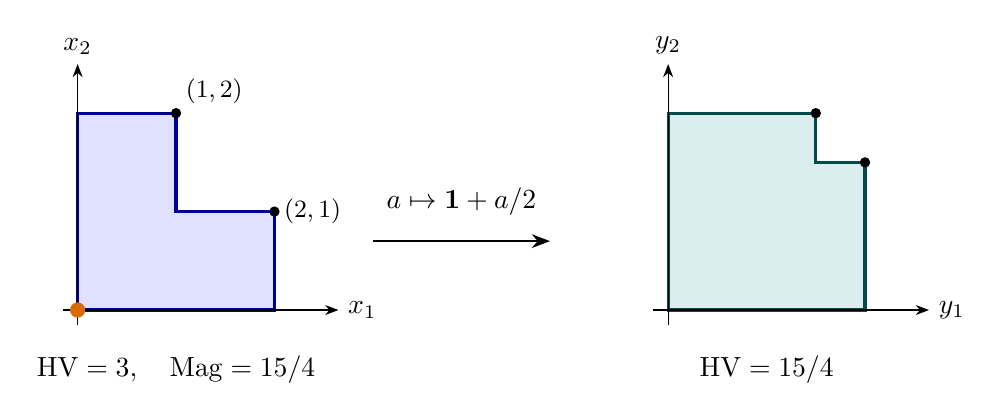
\begin{tikzpicture}[scale=1.25,>=Stealth]
 \begin{scope}
 \fill[blue!12] (0,0)--(2,0)--(2,1)--(1,1)--(1,2)--(0,2)--cycle;
 \draw[very thick,blue!60!black] (0,0)--(2,0)--(2,1)--(1,1)--(1,2)--(0,2)--cycle;
 \draw[->] (-.15,0)--(2.65,0) node[right] {$x_1$};
 \draw[->] (0,-.15)--(0,2.5) node[above] {$x_2$};
 \fill (2,1) circle(1.5pt) node[right] {\small$(2,1)$};
 \fill (1,2) circle(1.5pt) node[above right] {\small$(1,2)$};
 \fill[orange!85!black] (0,0) circle(2.2pt);
 \node at (1,-.6) {$\HV=3,\quad\Mag=15/4$};
 \end{scope}
 \node at (3.9,1.1) {$a\mapsto\ind+a/2$};
 \draw[->,thick] (3,0.7)--(4.8,0.7);
 \begin{scope}[xshift=6cm]
 \fill[teal!14] (0,0)--(2,0)--(2,1.5)--(1.5,1.5)--(1.5,2)--(0,2)--cycle;
 \draw[very thick,teal!60!black] (0,0)--(2,0)--(2,1.5)--(1.5,1.5)--(1.5,2)--(0,2)--cycle;
 \draw[->] (-.15,0)--(2.65,0) node[right] {$y_1$};
 \draw[->] (0,-.15)--(0,2.5) node[above] {$y_2$};
 \fill (2,1.5) circle(1.5pt);
 \fill (1.5,2) circle(1.5pt);
 \node at (1,-.6) {$\HV=15/4$};
 \end{scope}
\end{tikzpicture}
\caption{The transformed generators define a new anchored region. The
left region's magnitude equals the right region's ordinary area. The
origin atom and lower-dimensional contributions are represented by the
enlargement of anchored extents, not by a translation of the shaded set.}
\label{fig:shift}
\end{figure}


\subsection{Using the same numerical engine}
\label{app:magnitude-software}

On the cells of Section~\ref{sec:discrete}, the initial masses are
\[
 w_i(0)=1,\qquad w_i(k)=\frac{c_{i,k}-c_{i,k-1}}2\quad(k\ge1).
\]
Replacing the Lebesgue masses by these masses changes neither the cutoff
algebra nor the recursion. Prefix sums include the original origin atom.
Cropping shifts rank indices only: it must not insert a new atom at the
new rank zero. Compression adds existing cell masses, including atoms;
it does not reconstruct a continuous density by dividing by cell volume.
The hypotheses of Theorem~\ref{thm:main} therefore apply. Alternatively,
one can transform the generators by~\eqref{eq:forward} and call an ordinary
HV solver. Neither route improves the asymptotic exponent.

For Example~\ref{ex:two-box}, the axis coordinates are $(0,1,2)$.
The HV masses are $(0,1,1)$ and the magnitude masses are $(1,1/2,1/2)$.
The only uncovered cell in the enclosing rank grid is $(2,2)$, giving
HV $4-1=3$ and magnitude $4-1/4=15/4$.

The public interface also supports the indicator directly:
\begin{lstlisting}[language=Python]
from NumericalChanHVND.numerical_chan_local_compiled import magnitude
points = [(2, 1, 1, 1), (1, 2, 1, 1)]
assert abs(magnitude(points) - 135.0 / 16.0) < 1e-10
\end{lstlisting}
Here $(15/4)(3/2)^2=135/16$. An empty input has magnitude zero, whereas
a single all-zero generator has magnitude one. Zero-extent boxes must
therefore be retained for this application. The reflection from a
minimization region to upper-corner extents is an $\ell_1$ isometry, so
it also preserves the metric magnitude of the corresponding region.

The saved validation record includes 18 checks of the two HV--magnitude
transformations. The 64-point checkpoint instance and both checkpoint
decisions were also checked for magnitude against transformed Chan $d/2$
inputs. The 1,552-box instance has magnitude $411\,863\,688.75$, again
agreeing with the transformed reference. The shared algebra tests include
boundary atoms. These are correctness checks, not evidence that magnitude
improves the running time of ordinary HV. The larger benchmark in
Section~\ref{sec:experiments} measures ordinary hypervolume only.

\clearpage
\section{A worked eight-point example in 4D}
\label{app:eight}

This example explains the numerical objects before using them. A
\emph{cell} is a small rectangular region on which box membership is
constant. Its \emph{mass} is its ordinary volume. A \emph{mask} is a
zero-or-one rule that excludes a covered region. A \emph{contraction}
means summing out a coordinate. \emph{Compression} means grouping
consecutive coordinate cells and retaining their total masses, together
with any dependence between coordinates.

\subsection{Input, reference point, and the two projections}
Use the origin as anchor and interpret the following points as upper
corners: larger coordinates are better. Equivalently, for minimization
with reference $r=(6,6,6,6)$, use objective vectors $p^j=r-a^j$.
All coordinates of both sets lie in $\{1,2,3,4,5\}$.
\begin{center}
\begin{tabular}{@{}c@{\qquad}rrrr@{\qquad}c@{}}
\toprule
Point & $a_1$ & $a_2$ & $a_3$ & $a_4$ & Coordinate sum\\\midrule
$a^1$ &5&1&5&1&12\\
$a^2$ &5&2&3&2&12\\
$a^3$ &4&3&4&1&12\\
$a^4$ &3&4&2&3&12\\
$a^5$ &2&5&1&4&12\\
$a^6$ &1&5&2&4&12\\
$a^7$ &2&2&5&3&12\\
$a^8$ &1&3&3&5&12\\\bottomrule
\end{tabular}
\end{center}
No point dominates another: distinct vectors with the same coordinate
sum cannot be coordinatewise larger than one another. Their boxes
nevertheless overlap. The enclosing box is $[0,5]^4$, of volume $625$.

\begin{figure}[h!]
\centering
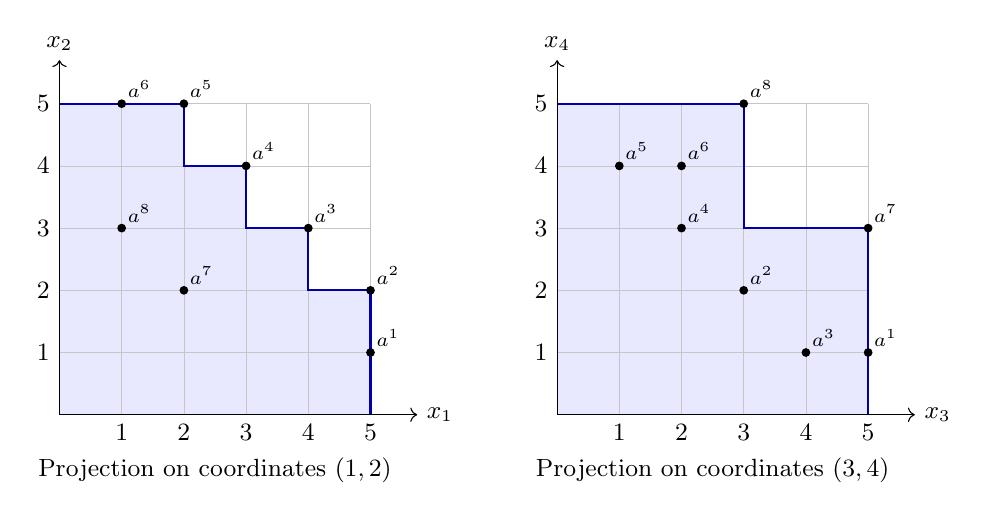
\begin{tikzpicture}[scale=.79, every node/.style={font=\small}]
\begin{scope}
\fill[blue!9] (0,0)--(5,0)--(5,2)--(4,2)--(4,3)--(3,3)--(3,4)--(2,4)--(2,5)--(0,5)--cycle;
\draw[step=1,gray!45,very thin] (0,0) grid (5,5);
\draw[blue!65!black,thick] (5,0)--(5,2)--(4,2)--(4,3)--(3,3)--(3,4)--(2,4)--(2,5)--(0,5);
\draw[->] (0,0)--(5.75,0) node[right] {$x_1$};
\draw[->] (0,0)--(0,5.7) node[above] {$x_2$};
\foreach \k in {1,...,5} {\node[below] at (\k,0) {\k};\node[left] at (0,\k) {\k};}
\foreach \x/\y/\lab in {5/1/1,5/2/2,4/3/3,3/4/4,2/5/5,1/5/6,2/2/7,1/3/8}
{\fill (\x,\y) circle (2pt);\node[above right,inner sep=2pt] at (\x,\y) {\scriptsize $a^{\lab}$};}
\node at (2.5,-.9) {Projection on coordinates $(1,2)$};
\end{scope}
\begin{scope}[xshift=8cm]
\fill[blue!9] (0,0)--(5,0)--(5,3)--(3,3)--(3,5)--(0,5)--cycle;
\draw[step=1,gray!45,very thin] (0,0) grid (5,5);
\draw[blue!65!black,thick] (5,0)--(5,3)--(3,3)--(3,5)--(0,5);
\draw[->] (0,0)--(5.75,0) node[right] {$x_3$};
\draw[->] (0,0)--(0,5.7) node[above] {$x_4$};
\foreach \k in {1,...,5} {\node[below] at (\k,0) {\k};\node[left] at (0,\k) {\k};}
\foreach \x/\y/\lab in {5/1/1,3/2/2,4/1/3,2/3/4,1/4/5,2/4/6,5/3/7,3/5/8}
{\fill (\x,\y) circle (2pt);\node[above right,inner sep=2pt] at (\x,\y) {\scriptsize $a^{\lab}$};}
\node at (2.5,-.9) {Projection on coordinates $(3,4)$};
\end{scope}
\end{tikzpicture}
\caption{Each label refers to the same 4D point in both plots. Shading
shows the union of projected anchored rectangles. Its areas are $19$
and $21$, respectively. Their product, $399$, is not the 4D hypervolume.}
\label{fig:eight-projections}
\end{figure}
\clearpage
\subsection{A hand-checkable calculation using the $2+2$ grouping}
The projections discard which pair belongs with which other pair.
For example, cell $(5,2)$ belongs to the left projection and cell $(3,5)$
to the right, but no input point covers the 4D cell $(5,2,3,5)$.

Every axis has coordinates $0,1,2,3,4,5$. For positive rank $k$ the cell
is $(k-1,k]$ and its length is $1$. The endpoint cell $\{0\}$ has
length zero and may be omitted in this ordinary-HV calculation.
Thus a positive-rank 4D cell has volume $1$.

Fix ranks $(i,j)$ in coordinates $(1,2)$. Only points with
$a_1\ge i$ and $a_2\ge j$ cover that first pair of cells. Let
\[
 H(i,j)=\HV_2\bigl(\{(a_3,a_4):a\in A,\ a_1\ge i,\ a_2\ge j\}\bigr).
\]
This is the area covered in the other two coordinates, conditional on
the chosen first pair. The word ``conditional'' here means selecting
the eligible points; it does not refer to a probability distribution.
All first-pair cells have area $1$, so
\[
                    \HV_4(A)=\sum_{i=1}^5\sum_{j=1}^5 H(i,j).
\]
The table can be checked by drawing the eligible rectangles in the
right-hand plot of Figure~\ref{fig:eight-projections}:
\begin{center}
\begin{tabular}{@{}c|rrrrr|r@{}}
\toprule
 & $j=1$&$j=2$&$j=3$&$j=4$&$j=5$&Row sum\\\midrule
$i=1$&21&21&16&8&8&74\\
$i=2$&16&16&9&7&4&52\\
$i=3$&10&9&8&6&0&33\\
$i=4$&8&7&4&0&0&19\\
$i=5$&8&6&0&0&0&14\\\bottomrule
\end{tabular}
\end{center}
For example, at $(i,j)=(2,3)$ the eligible points are $a^3,a^4,a^5$.
Their last two coordinates are $(4,1),(2,3),(1,4)$.
In the $x_3$ direction, the covered heights in $x_4$ are $4,3,1,1,0$.
Therefore $H(2,3)=4+3+1+1=9$. At $(5,2)$ only $a^2$ remains, and
$H(5,2)=3\cdot2=6$. Summing the rows gives
\[
               \boxed{\HV_4(A)=74+52+33+19+14=192.}
\]

\paragraph{What replaces integration?}
Let $W(t)=\sum_{s=1}^t1=t$, with $W(0)=0$. This is a prefix sum:
one stored cumulative mass for every endpoint. An interval of ranks
$q,\ldots,h$ has mass $W(h)-W(q-1)$ when $q\le h$, and zero otherwise.
It is exactly the integral of the unit density over those cells.
For instance, ranks $2,3$ have mass $W(3)-W(1)=3-1=2$.
No approximation of a continuous integral is involved.

The table above is an independent explanation and check, not the
data structure used by the fast algorithm. Constructing every such
table for a large input would not establish Chan's bound. The numerical
solver instead stores separate arrays and constraints and sums them
within the geometric recursion, as shown next.

\clearpage
\subsection{The actual recursion and its first absorbed box}
The solver computes the \emph{uncovered} volume $U$ inside $[0,5]^4$
and returns $625-U$. A simple box can be absorbed into a mask: the
box is removed from the list, while the mask remembers precisely which
cells must be excluded from subsequent sums.

At the root, $a^1=(5,1,5,1)$ reaches the enclosing boundary on axes
1 and 3. Only coordinates 2 and 4 restrict its coverage. On positive
ranks, its complement is
\[
 F(k)=\ind[k_2>1\ \text{or}\ k_4>1]
     =\ind[k_4\ge q(k_2)],\qquad
 q(j)=\begin{cases}2,&j=1,\\1,&j=2,3,4,5.\end{cases}
\]
The remaining seven boxes are initially hard: each still restricts at
least three coordinates. The prefix-sum calculation must keep $F$;
otherwise cells covered by $a^1$ would be counted as uncovered.

With the default base size of two hard boxes, the local compiled solver
chooses the following cuts. $L$ and $R$ mean the lower and upper child
of a cut. The table gives original positive ranks, rather than the
shifted local indices used internally after cropping arrays. A star
means the full positive range $1{:}5$.
\begin{center}
\small
\begin{tabular}{@{}lccccrl@{}}
\toprule
Node&$k_1$&$k_2$&$k_3$&$k_4$&$U$&Next operation\\\midrule
Root&$*$&$*$&$*$&$*$&433&Cut axis 1 after 3\\
$L$&$1{:}3$&$*$&$*$&$*$&216&Cut axis 2 after 3\\
$LL$&$1{:}3$&$1{:}3$&$*$&$*$&99&Cut axis 3 after 2\\
$LLL$&$1{:}3$&$1{:}3$&$1{:}2$&$*$&21&Base, two hard boxes\\
$LLR$&$1{:}3$&$1{:}3$&$3{:}5$&$*$&78&Base, two hard boxes\\
$LR$&$1{:}3$&$4{:}5$&$*$&$*$&117&Cut axis 3 after 2\\
$LRL$&$1{:}3$&$4{:}5$&$1{:}2$&$*$&27&Base, one hard box\\
$LRR$&$1{:}3$&$4{:}5$&$3{:}5$&$*$&90&Base, no hard boxes\\
$R$&$4{:}5$&$*$&$*$&$*$&217&Base, two hard boxes\\\bottomrule
\end{tabular}
\end{center}
These are the weighted-median cuts of Section~\ref{sec:geometry},
recorded from the implementation, not a separately chosen sweep.
For example, $99=21+78$, $117=27+90$, and $216=99+117$.
At the root, $U=216+217=433$, giving $625-433=192$.

There are four cuts, nine visited nodes, and five base evaluations.
After a cut, more boxes may become simple because they reach a new
cell boundary. Their masks remain in the numerical state even after
their generators leave the hard-box list. The table's $U$ is the
original uncovered volume in that region, including all inherited masks.
This small instance finishes before any scheduled compression occurs.
We illustrate compression separately below rather than claiming that
this run exercises it.

\clearpage
\subsection{One complete leaf calculation using numerical arrays}
Consider node $R$, where $k_1\in\{4,5\}$. Points $a^4,\ldots,a^8$
are disjoint from this region because their first coordinate is at most
3. Box $a^1$ has already become the mask $F$. Only $a^2$ and $a^3$
remain as hard boxes.

For any rank rectangle $E$ in this node, write
$M(E)=\sum_{k\in E}F(k)$. This is a sum of unit masses, excluding the
cells covered by $a^1$. To evaluate it, sum coordinate 4 first. For
each allowed $j=k_2$ and upper fourth rank $h$, the result is
\[
 S(j,h)=\begin{cases}W(h)-W(q(j)-1),&h\ge q(j),\\0,&h<q(j).
 \end{cases}
\]
The zero case is important: an empty interval contributes zero, never
a negative volume. The remaining sums multiply by the numbers of
allowed first and third ranks. This is numerical elimination: one
coordinate is replaced by an array of its summed values.

\begin{center}
\begin{tabular}{@{}lrrrrl@{}}
\toprule
Restriction&$\#k_1$&$h_2$&$h_3$&$h_4$&$M(E)$\\\midrule
None&2&5&5&5&$2\cdot5\,(4+5+5+5+5)=240$\\
Inside $a^2$&2&2&3&2&$2\cdot3\,(1+2)=18$\\
Inside $a^3$&1&3&4&1&$1\cdot4\,(0+1+1)=8$\\
Inside both&1&2&3&1&$1\cdot3\,(0+1)=3$\\\bottomrule
\end{tabular}
\end{center}
Here $h_2,h_3,h_4$ are the upper ranks in the last three coordinates;
their lower ranks are 1. The first-coordinate counts already include
intersection with $\{4,5\}$. For example, $a^3$ allows only $k_1=4$.

To exclude both remaining boxes, use
\[
 (1-\ind_{a^2})(1-\ind_{a^3})
   =1-\ind_{a^2}-\ind_{a^3}+\ind_{a^2\cap a^3}.
\]
The overlap is added back because it was subtracted twice. Hence
\[
                      U_R=240-18-8+3=217.
\]
This leaf region has volume $2\cdot5^3=250$, so its covered volume is
$250-217=33$. The first table independently gives $19+14=33$ for rows
$i=4,5$.

The base calculation expands only the two hard boxes left at this node,
giving four terms. It does not expand all $2^8$ subsets of the original
input. On larger inputs the fixed base size still bounds this number.
All operations displayed here are array lookups, additions,
subtractions and multiplications. Chan's integral formulation and this
finite calculation evaluate the same quantity; their stored objects differ.

\clearpage
\subsection{What compression would retain in this leaf}
For illustration only, group ranks using the boundaries of the two
remaining hard boxes. On axis 2, use blocks $\{1,2\},\{3\},\{4,5\}$;
on axis 4, use $\{1\},\{2\},\{3,4,5\}$. On axis 1 keep $\{4\},\{5\}$,
and on axis 3 use $\{1,2,3\},\{4\},\{5\}$. Neither remaining box
cuts the interior of any block. This is why their later membership
tests can operate on block indices.

The earlier mask from $a^1$ does cut through the first axis-2 block.
We therefore sum its values within each pair of blocks, rather than
discarding it. The resulting masses for axes $(2,4)$ are
\begin{center}
\begin{tabular}{@{}c|rrr@{}}
\toprule
Axis-2 block $\backslash$ axis-4 block&$\{1\}$&$\{2\}$&$\{3,4,5\}$\\\midrule
$\{1,2\}$&1&2&6\\
$\{3\}$&1&1&3\\
$\{4,5\}$&2&2&6\\\bottomrule
\end{tabular}
\end{center}
The upper-left entry is $1$, because $(k_2,k_4)=(1,1)$ is excluded but
$(2,1)$ is allowed. The entry $6$ in the first row counts all
$2\cdot3$ pairs in $\{1,2\}\times\{3,4,5\}$.
The entries sum to $24$; multiplying by the first- and third-axis
lengths gives $2\cdot5\cdot24=240$ again.

The hard-box restrictions now give exactly the same three other masses:
\[
 M(a^2)=2\cdot3\,(1+2)=18,\qquad
 M(a^3)=1\cdot4\,(1+1)=8,\qquad
 M(a^2\cap a^3)=1\cdot3\cdot1=3.
\]
Thus compression preserves the leaf answer $217$. But the table is
not a product of one axis-2 array and one axis-4 array: its upper-left
$2\times2$ determinant is $1\cdot1-2\cdot1=-1$, whereas such a product
would have determinant zero. The coupling created by the mask survives
compression. In this special case it can be written as
\[
 \begin{pmatrix}2\\1\\2\end{pmatrix}
 \begin{pmatrix}1&1&3\end{pmatrix}
 -
 \begin{pmatrix}1\\0\\0\end{pmatrix}
 \begin{pmatrix}1&0&0\end{pmatrix}.
\]
This is a sum of two products with a negative coefficient, even though
every final block mass is nonnegative. The general algorithm stores
sums of products with pair constraints, not dense tables of all block
combinations. This small table only makes the preserved information visible.

\paragraph{Reproducing and interpreting the check.}
The companion script \path{eight_point_example.py} checks the 625 unit cells,
all subset intersections, the planar table, the leaf formulas, and the
compressed masses using integers. With \texttt{--compiled} it also checks
the exact numerical solver and records the compiled solver's recursion.
Run it from the repository root as
\begin{lstlisting}
python NumericalChanHVND/paper/eight_point_example.py --compiled
\end{lstlisting}
The saved record is \path{eight_point_example.json}. Agreement on this
example explains and tests the formulas; it does not prove the complexity
bound. The full bound also needs the accounting of branching, stored
array lengths, and repeated compression in Theorem~\ref{thm:main}.

\clearpage
\section{A compact implementation and proof map}
\label{app:map}

The following table locates the main mathematical obligations. The names
refer to files in \texttt{NumericalChanHVND}; the proof specifies exact
arithmetic while the compiled code evaluates the same formulas in binary64.
\begin{center}
\small
\begin{tabularx}{\linewidth}{@{}>{\raggedright\arraybackslash}p{.28\linewidth}>{\raggedright\arraybackslash}X@{}}
\toprule
Mathematical operation & Implementation location and invariant\\\midrule
Axis cells and masses & \texttt{numerical\_chan\_numba.py},
\texttt{compute}: interval lengths for HV; ranks preserve box membership.\\
Cell simplification & \texttt{numerical\_chan\_compiled.py},
\texttt{\_cell\_state}: disjointness, slab tightening, cropping and pair masks.\\
Scalar contraction & \texttt{compiled\_terms.py},
\texttt{eliminate}: first-winner guards and signed prefix differences.\\
Block compression & \texttt{compiled\_terms.py},
\texttt{push\_blocks}: lift to $2d$ variables, eliminate old axes, retain block masses.\\
Local schedule & \texttt{numerical\_chan\_local\_compiled.py},
\texttt{\_node} and \texttt{\_new\_block}: one budget step per cyclic advance;
restart at every checkpoint.\\
Validation & \texttt{verify\_compiled.py} checks the shared algebra;
\texttt{verify\_local\_compiled.py} adds local scheduling and end-to-end checks.\\
\bottomrule
\end{tabularx}
\end{center}

The larger experiment uses \texttt{benchmarks/larger\_4d\_6d}, with
saved coordinates, every retained repetition, partial runs and source
hashes. Its unchanged solver sources are from revision \texttt{095fa73}.
The earlier experiment remains in \texttt{benchmarks/compiled\_2d\_10d},
including its exact-oracle record and natural-compression probe. Revision
\texttt{38587e7} identifies that earlier release. The local driver is now
timed explicitly in the larger comparison; old speedup ratios are not
transferred to it.

To reproduce correctness and build this manuscript from the repository
root, use the following commands. LaTeX is run in the paper directory
because the experimental sections and appendices are companion source files.
\begin{lstlisting}
python NumericalChanHVND/verify_local_compiled.py
cd NumericalChanHVND/paper
pdflatex -interaction=nonstopmode -halt-on-error numerical_product_chan.tex
pdflatex -interaction=nonstopmode -halt-on-error numerical_product_chan.tex
\end{lstlisting}
The report uses the standard article class, A4 paper, 12-point text, and
an inline \texttt{thebibliography} with \texttt{bibitem} entries. It can
be compiled without a bibliography database or code execution by LaTeX.

\clearpage
\begin{thebibliography}{9}
\raggedright
\bibitem{chan2013}
Timothy M. Chan.
\newblock Klee's Measure Problem Made Easy.
\newblock In \emph{Proceedings of the 54th Annual IEEE Symposium on
Foundations of Computer Science (FOCS)}, pages 410--419, 2013.
\newblock \url{https://doi.org/10.1109/FOCS.2013.51}.
\newblock Author version, 10 August 2013:
\url{https://tmc.web.engr.illinois.edu/easyklee8_13.pdf}.

\bibitem{zitzlerthiele1998}
Eckart Zitzler and Lothar Thiele.
\newblock Multiobjective optimization using evolutionary algorithms---A
comparative case study.
\newblock In \emph{Parallel Problem Solving from Nature---PPSN V},
volume 1498 of \emph{Lecture Notes in Computer Science}, pages 292--301.
Springer, Berlin, Heidelberg, 1998.
\newblock \url{https://doi.org/10.1007/BFb0056872}.

\bibitem{wikipediahv}
Wikipedia contributors.
\newblock Hypervolume indicator.
\newblock \emph{Wikipedia, The Free Encyclopedia}.
\newblock \url{https://en.wikipedia.org/wiki/Hypervolume_indicator}.
Accessed 5 October 2026.

\bibitem{emmerich2026}
Michael T. M. Emmerich.
\newblock The Magnitude of Dominated Sets: A Pareto Compliant Indicator
Grounded in Metric Geometry.
\newblock arXiv:2604.18147v1, 2026.
\newblock \url{https://doi.org/10.48550/arXiv.2604.18147}.

\bibitem{leinstermeckes2017}
Tom Leinster and Mark W. Meckes.
\newblock The magnitude of a metric space: from category theory to
geometric measure theory.
\newblock In Nicola Gigli, editor, \emph{Measure Theory in Non-Smooth
Spaces}, pages 156--193. De Gruyter, 2017.
\newblock \url{https://doi.org/10.1515/9783110550832-005}.
\newblock Preprint: \url{https://arxiv.org/abs/1606.00095}.

\bibitem{emmerichdeutz2018}
Michael T. M. Emmerich and Andr\'e H. Deutz.
\newblock A tutorial on multiobjective optimization: fundamentals and
evolutionary methods.
\newblock \emph{Natural Computing}, 17:585--609, 2018.
\newblock \url{https://doi.org/10.1007/s11047-018-9685-y}.

\bibitem{magnitudesoftware}
Michael T. M. Emmerich.
\newblock Pair-Elimination and Product-Measure Simplification of
Chan's Fixed-Dimensional Hypervolume Algorithm.
\newblock Working research note, 2 October 2026, in the
\texttt{HV4DMagnitude} repository.
\newblock \href{https://github.com/emmerichmtm/HV4DMagnitude/blob/main/paper/magnitude_chan_pair_elimination_report.pdf}{Report PDF};
\href{https://github.com/emmerichmtm/HV4DMagnitude/blob/main/paper/magnitude_chan_pair_elimination_report.tex}{LaTeX source}.
\newblock \url{https://github.com/emmerichmtm/HV4DMagnitude}.

\bibitem{software}
\emph{FastHVChan: numerical hypervolume and magnitude implementations}.
\newblock Repository of Michael Emmerich, including
\texttt{NumericalChanHV4D} and \texttt{NumericalChanHVND}.
\newblock Solver releases: \texttt{38587e7} (archived small-input
benchmark) and \texttt{095fa73} (larger 4D--6D comparison), 4 October 2026.
\newblock Complete source hashes and samples: accompanying
\texttt{NumericalChanHVND} benchmark files.
\newblock \url{https://github.com/emmerichmtm/FastHVChan}.
\end{thebibliography}
\end{document}
